\documentclass[compress]{beamer}

\usepackage[T1,T2A]{fontenc}
\usepackage[utf8]{inputenc}
\usepackage[english,russian]{babel}
\usepackage{hyperref}
\usepackage{microtype}
\usepackage{csquotes}
\usepackage{amsmath}
\usepackage{amsthm}
\usepackage{amssymb}
\usepackage{mathtext}
\usepackage{physics}
\usepackage{newfloat}
\usepackage{caption}
\usepackage{indentfirst}
\usepackage{hyperref}
\usepackage{mdframed}
\usepackage{graphicx}
\usepackage{subfig}
\usepackage{appendix}

%% workaround for the \@ifundefined macro update in the 2018 LaTeX release
%% should be fixed in one of the next releases of caption.sty
\makeatletter
\let\@@magyar@captionfix\relax
\makeatother

\DeclareGraphicsExtensions{.pdf,.png,.jpg,.PNG}
\graphicspath{{./img/}}
\captionsetup[figure]{justification=centering}
\renewcommand{\thesubfigure}{\asbuk{subfigure}}
\DeclareCaptionLabelSeparator{dotseparator}{. }
\captionsetup{labelsep=dotseparator}
\makeatletter\appto{\appendices}{\def\Hy@chapapp{Appendix}}\makeatother
\renewcommand{\appendixtocname}{Приложения}
\renewcommand{\appendixpagename}{Приложения}
\setbeamertemplate{background canvas}[vertical shading][bottom=red!2,top=green!2]

\usetheme{Ilmenau}
\usecolortheme{spruce}
\usefonttheme[onlysmall]{serif}

\setbeamercolor{title in head/foot}{parent=palette primary}
\setbeamercolor{author in head/foot}{parent=palette primary}
\setbeamercolor{institute in head/foot}{parent=palette primary}

\setbeamercolor{title}{fg=black}
\setbeamercolor{frametitle}{fg=black}
\setbeamercolor*{enumerate item}{fg=black}

\setbeamercolor*{bibliography item}{fg=black}
\setbeamercolor*{bibliography entry title}{fg=black}
\setbeamercolor*{bibliography entry author}{fg=black}
\setbeamercolor*{bibliography entry location}{fg=black}
\setbeamercolor*{bibliography entry note}{fg=black}

\setbeamertemplate{enumerate item}[default]
\setbeamertemplate{bibliography entry title}{}
\setbeamertemplate{bibliography entry location}{}
\setbeamertemplate{bibliography entry note}{}
\setbeamertemplate{bibliography item}{\insertbiblabel}

\addtobeamertemplate{navigation symbols}{}{%
    \usebeamerfont{footline}%
    \usebeamercolor[fg]{title}%
    \hspace{1em}%
    \insertframenumber/\inserttotalframenumber
}

\hypersetup{
    colorlinks,
    citecolor=black,
    filecolor=black,
    linkcolor=black,
    urlcolor=black
}

\AtBeginSection[]{
  \begin{frame}
  \vfill
  \centering
  \begin{beamercolorbox}[sep=8pt,center,shadow=true,rounded=true]{title}
    \usebeamerfont{title}\insertsection\par%
  \end{beamercolorbox}
  \vfill
  \end{frame}
}

\DeclareMathOperator{\Rot}{\mathbf{rot}}
\DeclareMathOperator{\Grad}{\mathbf{grad}}
\DeclareMathOperator{\Div}{\mathbf{div}}
\DeclareMathOperator{\D}{D}
\newcommand{\V}[1]{\mathbf{#1}}
\newcommand{\Op}[1]{\hat{\V{#1}}}


\graphicspath{{./img/}{../../fragments/math/img/}{../../fragments/spherical_modes/img/}{../../fragments/spherical_resonators/img/}{../../fragments/thermodynamics/img/}}

\deftranslation[to=russian]{Theorem}{Теорема}
\deftranslation[to=russian]{theorem}{Теорема}

\title{Тепловое излучение\\ в сферическом резонаторе}
\author[Василевский~А.В.]{
    Василевский~А.В. \\[\baselineskip]
    {\footnotesize Научный руководитель: Бурланков~Д.Е.}
}
\institute[ННГУ]{Нижегородский университет им. Н.И.~Лобачевского}
\date{2018}

\begin{document}

    %
    %
    %
    %%%%%%%%%%%%%%%%%%%%%%%%%%%%%%%%%%%%%%%%%%%%%%%%%%%%%%%%%%%%%%%%%%%%%%%
    %                            FRAME                                    %
    %%%%%%%%%%%%%%%%%%%%%%%%%%%%%%%%%%%%%%%%%%%%%%%%%%%%%%%%%%%%%%%%%%%%%%%
    %
    %
    %

    \frame[plain]{\titlepage}

    %
    %
    %
    %%%%%%%%%%%%%%%%%%%%%%%%%%%%%%%%%%%%%%%%%%%%%%%%%%%%%%%%%%%%%%%%%%%%%%%
    %                            SECTION                                  %
    %%%%%%%%%%%%%%%%%%%%%%%%%%%%%%%%%%%%%%%%%%%%%%%%%%%%%%%%%%%%%%%%%%%%%%%
    %
    %
    %

    \section[Введение]{Введение и постановка задачи}

    %
    %
    %
    %%%%%%%%%%%%%%%%%%%%%%%%%%%%%%%%%%%%%%%%%%%%%%%%%%%%%%%%%%%%%%%%%%%%%%%
    %                            FRAME                                    %
    %%%%%%%%%%%%%%%%%%%%%%%%%%%%%%%%%%%%%%%%%%%%%%%%%%%%%%%%%%%%%%%%%%%%%%%
    %
    %
    %

    \begin{frame}\frametitle{Введение}

        \begin{itemize}

            \item Резонаторы в современной науке имеют важнейшее значение. Одним из ключевых направлений развития физики сегодня является квантовая теория измерений и связанный с ней интерес к манипуляциям с отдельными квантовыми объектами.

            \item В связи с обнаружением сверхузких резонансов рассеяния и возможностью создания на этой основе микрорезонаторов с гигантской добротностью, интерес к этому вопросу усилился многократно.

            \item Анализ различных характеристик резонаторов и путей диссипации энергии в них является задачей, требующей особого внимания.

        \end{itemize}

    \end{frame}

    %
    %
    %
    %%%%%%%%%%%%%%%%%%%%%%%%%%%%%%%%%%%%%%%%%%%%%%%%%%%%%%%%%%%%%%%%%%%%%%%
    %                            FRAME                                    %
    %%%%%%%%%%%%%%%%%%%%%%%%%%%%%%%%%%%%%%%%%%%%%%%%%%%%%%%%%%%%%%%%%%%%%%%
    %
    %
    %

    \begin{frame}\frametitle{Оптический микрорезонатор с МШГ}

        \begin{figure}[h]
            \centering
            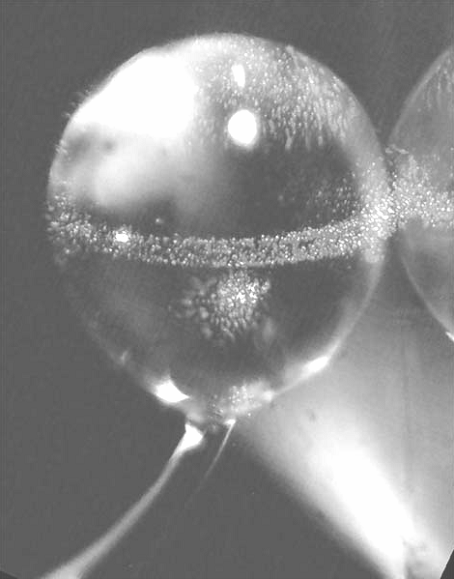
\includegraphics[width=\textwidth,height=0.6\textheight,keepaspectratio]{spherical_resonator}
            \caption[]{Оптический сферический микрорезонатор на ножке рядом с возбуждающей призмой, в которой видно его отражение. Диаметр около $570$ мкм, добротность $> 10^9$. Физический факультет МГУ \cite{microresonators}}
            \label{fig:spherical_resonator}
        \end{figure}

    \end{frame}

    %
    %
    %
    %%%%%%%%%%%%%%%%%%%%%%%%%%%%%%%%%%%%%%%%%%%%%%%%%%%%%%%%%%%%%%%%%%%%%%%
    %                            FRAME                                    %
    %%%%%%%%%%%%%%%%%%%%%%%%%%%%%%%%%%%%%%%%%%%%%%%%%%%%%%%%%%%%%%%%%%%%%%%
    %
    %
    %

    \begin{frame}\frametitle{Постановка задачи}

        \textbf{Цели работы}:
        %
        \begin{itemize}
            \item \textbf{Описание электромагнитного поля внутри резонатора}.
                Применен подход, в основе которого лежат векторы Киллинга объемлющего пространства.
            \item \textbf{Описание спектральной плотности запасенной в резонаторе энергии}.
                Численно получена спектральная кривая, ложащаяся на планковскую.
        \end{itemize}

        \textbf{Физическая модель резонатора}:
        %
        \begin{itemize}
            \item Идеально сферический радиуса $r_\text{шара}$.
            \item Заполнен изотропным однородным диэлектриком.
            \item Стенки идеально проводящие.
        \end{itemize}

    \end{frame}

    %
    %
    %
    %%%%%%%%%%%%%%%%%%%%%%%%%%%%%%%%%%%%%%%%%%%%%%%%%%%%%%%%%%%%%%%%%%%%%%%
    %                            FRAME                                    %
    %%%%%%%%%%%%%%%%%%%%%%%%%%%%%%%%%%%%%%%%%%%%%%%%%%%%%%%%%%%%%%%%%%%%%%%
    %
    %
    %

    \begin{frame}\frametitle{Волновое уравнение}

        \begin{itemize}

            \item Основное уравнение задачи~--- волновое уравнение для комплексной амплитуды вектора напряженности $\V{E}$:
            %
            \begin{gather}
                \vb{E}_{osc} = \Re{\vb{E} \exp(-i \omega t)} \nonumber \\
                \Delta \V{E} = - \lambda \V{E} ; \quad
                    \lambda = \frac{\omega^2}{v^2} ; \quad
                    v = \frac{c}{\sqrt{\varepsilon\mu}} = \frac{c}{n} \label{eq:wave_equation}.
            \end{gather}

            \item Уравнение \autoref{eq:wave_equation}~--- уравнение на собственные функции и собственные значения (моды) оператора Лапласа $\Delta$.

            \item Граничные условия: $\vb{E}_\theta = \vb{E}_\varphi = 0$.

        \end{itemize}

    \end{frame}

    %
    %
    %
    %%%%%%%%%%%%%%%%%%%%%%%%%%%%%%%%%%%%%%%%%%%%%%%%%%%%%%%%%%%%%%%%%%%%%%%
    %                            FRAME                                    %
    %%%%%%%%%%%%%%%%%%%%%%%%%%%%%%%%%%%%%%%%%%%%%%%%%%%%%%%%%%%%%%%%%%%%%%%
    %
    %
    %

    \begin{frame}\frametitle{Решение волнового уравнения}

        \begin{itemize}

            \item Сопряжено со значительными трудностями.

            \item Классические подходы громоздки и не обобщаются на поля произвольной тензорной размерности \cite{burlankov_tmf}.

            \item Операторный вид уравнения позволяет эффективно применить теорию операторов.

            \item Подход, основанный на операторах Киллинга, коммутирующих с оператором Лапласа, может быть обобщен на произвольные пространства и поля \cite{burlankov_tmf}.

        \end{itemize}

    \end{frame}

    %
    %
    %
    %%%%%%%%%%%%%%%%%%%%%%%%%%%%%%%%%%%%%%%%%%%%%%%%%%%%%%%%%%%%%%%%%%%%%%%
    %                            FRAME                                    %
    %%%%%%%%%%%%%%%%%%%%%%%%%%%%%%%%%%%%%%%%%%%%%%%%%%%%%%%%%%%%%%%%%%%%%%%
    %
    %
    %

    \begin{frame}\frametitle{Операторный подход}

        \begin{itemize}

            \item $\Op{D}_1$, $\Op{D}_2$~--- дифференциальные операторы.

            \item $\qty[\Op{D}_1, \Op{D}_2] \tau = (\Op{D}_1\Op{D}_2 - \Op{D}_2\Op{D}_1) \tau = 0$~--- операторы коммутируют.

        \end{itemize}

        \begin{align*}
            \left. \begin{aligned}
                \qty[\Op{D}_1, \Op{D}_2] &= 0 \\
                \Op{D}_1 \tau &= \lambda_1 \tau
            \end{aligned} \right\}
            \quad \Longrightarrow \quad &
            \Op{D}_2 \tau = \lambda_2 \tau
        \end{align*}

    \end{frame}

    %
    %
    %
    %%%%%%%%%%%%%%%%%%%%%%%%%%%%%%%%%%%%%%%%%%%%%%%%%%%%%%%%%%%%%%%%%%%%%%%
    %                            SECTION                                  %
    %%%%%%%%%%%%%%%%%%%%%%%%%%%%%%%%%%%%%%%%%%%%%%%%%%%%%%%%%%%%%%%%%%%%%%%
    %
    %
    %

    \section[Методика]{Методика получения сферических мод}

    %
    %
    %
    %%%%%%%%%%%%%%%%%%%%%%%%%%%%%%%%%%%%%%%%%%%%%%%%%%%%%%%%%%%%%%%%%%%%%%%
    %                            FRAME                                    %
    %%%%%%%%%%%%%%%%%%%%%%%%%%%%%%%%%%%%%%%%%%%%%%%%%%%%%%%%%%%%%%%%%%%%%%%
    %
    %
    %

    \begin{frame}\frametitle{Операторы Киллинга}

        \begin{itemize}

            \item Ли-вариация $\delta_\xi\tau$~--- инвариантное обобщение производной по направлению на произвольные тензорные поля \cite{lie_derivative_theory,symmetry_and_killing_fields}.
            %
            \begin{equation*}\begin{aligned}
                \delta_\xi a^i &= \xi^c \partial_c a^i - a^c \partial_{c} \xi^i , \\
                \delta_\xi g_{ij} &= \nabla_i \xi_j + \nabla_j \xi_i .
            \end{aligned}\end{equation*}

            \item Метрический тензор $g_{ij}$ полностью определяет метрику риманова пространства.

            \item Если $\delta_\xi g_{ij} = 0$, то говорят, что $\xi$~--- поле Киллинга, или движение, а $\delta_\xi$~--- оператор Киллинга.

        \end{itemize}

    \end{frame}

    %
    %
    %
    %%%%%%%%%%%%%%%%%%%%%%%%%%%%%%%%%%%%%%%%%%%%%%%%%%%%%%%%%%%%%%%%%%%%%%%
    %                            FRAME                                    %
    %%%%%%%%%%%%%%%%%%%%%%%%%%%%%%%%%%%%%%%%%%%%%%%%%%%%%%%%%%%%%%%%%%%%%%%
    %
    %
    %

    \begin{frame}\frametitle{Поля Киллинга евклидова пространства}

        В трехмерном евклидовом пространстве существует шесть полей Киллинга. В декартовых координатах:
        %
        \begin{equation*}
            \V{\xi}_i
            =
            \left[
                \V{n}_x, \V{n}_y, \V{n}_z,
                \V{l}_x, \V{l}_y, \V{l}_z
            \right]
            =
            \begin{bmatrix}
                1 & 0 & 0 & 0  & -z & y  \\
                0 & 1 & 0 & z  & 0  & -x \\
                0 & 0 & 1 & -y & x  & 0
            \end{bmatrix}
        \end{equation*}

        Первая тройка образует группу движений трансляций, вторая~--- группу движений вращений.

    \end{frame}

    %
    %
    %
    %%%%%%%%%%%%%%%%%%%%%%%%%%%%%%%%%%%%%%%%%%%%%%%%%%%%%%%%%%%%%%%%%%%%%%%
    %                            FRAME                                    %
    %%%%%%%%%%%%%%%%%%%%%%%%%%%%%%%%%%%%%%%%%%%%%%%%%%%%%%%%%%%%%%%%%%%%%%%
    %
    %
    %

    \begin{frame}\frametitle{Поля Киллинга в сферических координатах}

        Группа вращений в сферической системе координат $(r,\theta,\varphi)$ в контравариантных компонентах:
        %
        \begin{equation*}
            \V{l}_i
            =
            \begin{bmatrix}
                0
                    & 0
                    & 0 \\
                \sin\varphi
                    & \cos\varphi
                    & 0 \\
                \cos\varphi \cot\theta
                    & \cot\theta \sin\varphi
                    & - 1
            \end{bmatrix}
            .
        \end{equation*}

         Следует отметить уже сейчас, что $\V{l}_z$ не зависит ни от одной из координат пространства, а также что ни один $\V{l}_i$ не содержит $r$-й компоненты.

    \end{frame}

    %
    %
    %
    %%%%%%%%%%%%%%%%%%%%%%%%%%%%%%%%%%%%%%%%%%%%%%%%%%%%%%%%%%%%%%%%%%%%%%%
    %                            FRAME                                    %
    %%%%%%%%%%%%%%%%%%%%%%%%%%%%%%%%%%%%%%%%%%%%%%%%%%%%%%%%%%%%%%%%%%%%%%%
    %
    %
    %

    \begin{frame}\frametitle{Производные операторы вращений}

        \begin{enumerate}
            \item Операторы Киллинга коммутируют с оператором Лапласа.

            \item Операторы вращений не коммутируют.

            \item Оператор $\Op{l}^2 = \Op{l}_x \Op{l}_x + \Op{l}_y \Op{l}_y + \Op{l}_z \Op{l}_z$ коммутирует со всеми операторами вращений.

            \item Операторы повышения и понижения, $\Op{l}_{+} = \Op{l}_x - i\Op{l}_y$ и $\Op{l}_{-} = \Op{l}_x + i\Op{l}_y$, также коммутируют с $\Op{l}^2$.
        \end{enumerate}

    \end{frame}

    %
    %
    %
    %%%%%%%%%%%%%%%%%%%%%%%%%%%%%%%%%%%%%%%%%%%%%%%%%%%%%%%%%%%%%%%%%%%%%%%
    %                            FRAME                                    %
    %%%%%%%%%%%%%%%%%%%%%%%%%%%%%%%%%%%%%%%%%%%%%%%%%%%%%%%%%%%%%%%%%%%%%%%
    %
    %
    %

    \begin{frame}\frametitle{Собственные моды операторов вращений}

        Пусть
        %
        \begin{equation*}\begin{gathered}
            \Op{l}^2 h_{l,m} = l (l + 1) h_{l,m} ; \quad
            \Op{l}_z h_{l,m} = i m h_{l,m} .
        \end{gathered}\end{equation*}

        Можно показать, что
        %
        \begin{equation*}\begin{gathered}
            \Op{l}_{+} h_{l,m} = h_{l,m+1} \\
            \Op{l}_{-} h_{l,m} = h_{l,m-1} ,
        \end{gathered}\end{equation*}
        %
        и что
        %
        \begin{equation*}\begin{gathered}
            \Op{l}_{+} h_{l,l} = 0 ; \quad
            \Op{l}_{-} h_{l,-l} = 0 ,
        \end{gathered}\end{equation*}
        %
        т.е. допустимо лишь $- l \le m \le l$.

    \end{frame}

    %
    %
    %
    %%%%%%%%%%%%%%%%%%%%%%%%%%%%%%%%%%%%%%%%%%%%%%%%%%%%%%%%%%%%%%%%%%%%%%%
    %                            FRAME                                    %
    %%%%%%%%%%%%%%%%%%%%%%%%%%%%%%%%%%%%%%%%%%%%%%%%%%%%%%%%%%%%%%%%%%%%%%%
    %
    %
    %

    \begin{frame}\frametitle{Базовые моды}

        Наиболее интересной является базовая мода, т.е. мода с $m = 0$, для которой
        %
        \begin{equation*}
            \Op{l}_z h_{l, 0} = \pdv{h_{l, 0}}{\varphi} = 0 .
        \end{equation*}
        %
        Базовая мода не зависит от $\varphi$. Кроме того, базовая мода удовлетворяет соотношению:
        %
        \begin{equation}\label{eq:basemode_eq}
            \Op{l}^2 h_{l, 0}
                = \qty( \Op{l}_{+} \Op{l}_{-} + \Op{l}_z^2 - i \Op{l}_z ) h_{l, 0}
                = \Op{l}_{+} \Op{l}_{-} h_{l, 0}
                = - l (l + 1) h_{l, 0} .
        \end{equation}
        %
        Но поскольку $\Op{l}_i$ не содержит $r$, уравнение \autoref{eq:basemode_eq} является уравнением только на $h_{l, 0}$ как функцию $\theta$.

    \end{frame}

    %
    %
    %
    %%%%%%%%%%%%%%%%%%%%%%%%%%%%%%%%%%%%%%%%%%%%%%%%%%%%%%%%%%%%%%%%%%%%%%%
    %                            FRAME                                    %
    %%%%%%%%%%%%%%%%%%%%%%%%%%%%%%%%%%%%%%%%%%%%%%%%%%%%%%%%%%%%%%%%%%%%%%%
    %
    %
    %

    \begin{frame}\frametitle{Методика нахождения сферических мод}

        \begin{enumerate}
            \item Построение базовых мод с $m = 0$ и определенным $l$ из \autoref{eq:basemode_eq}:
            %
            \begin{equation*}
                \Op{l}_{+} \Op{l}_{-} h_{l, 0} = - l (l + 1) h_{l, 0} .
            \end{equation*}
            %
            Результат~--- $h_{l, 0}$ с известной угловой частью и неизвестной радиальной.

            \item Нахождение радиальных функций для базовых мод из \autoref{eq:wave_equation}:
            %
            \begin{equation*}
                \Delta h_{l, 0} = - \lambda h_{l, 0} .
            \end{equation*}

            \item Получение остальных $2l$ производных мод с $m = \pm 1, \pm 2, \dots$ путем применения операторов повышения и понижения.

        \end{enumerate}

    \end{frame}

    %
    %
    %
    %%%%%%%%%%%%%%%%%%%%%%%%%%%%%%%%%%%%%%%%%%%%%%%%%%%%%%%%%%%%%%%%%%%%%%%
    %                            SECTION                                  %
    %%%%%%%%%%%%%%%%%%%%%%%%%%%%%%%%%%%%%%%%%%%%%%%%%%%%%%%%%%%%%%%%%%%%%%%
    %
    %
    %

    \section[Моды]{Нахождение векторных мод электромагнитного поля}

    %
    %
    %
    %%%%%%%%%%%%%%%%%%%%%%%%%%%%%%%%%%%%%%%%%%%%%%%%%%%%%%%%%%%%%%%%%%%%%%%
    %                            FRAME                                    %
    %%%%%%%%%%%%%%%%%%%%%%%%%%%%%%%%%%%%%%%%%%%%%%%%%%%%%%%%%%%%%%%%%%%%%%%
    %
    %
    %

    \begin{frame}\frametitle{Векторные моды}

        Операторы Киллинга применительно к векторным полям:
        %
        \begin{equation*}\label{eq:killing_operator}
            \Op{\xi} a^k
                \equiv \delta_\xi a^k
                = \xi^c \pdv{a^k}{x^c} - a^c \pdv{\xi^k}{x^c} .
        \end{equation*}

        Из-за наличия члена $a^c \pdv*{\xi^k}{x^c}$, пропорционального компонентам самого векторного поля, компоненты проварьированного на $\xi$ векторного поля $\vb{a}$ приобретают весьма сложный вид, что доставляет определенные трудности для прямого решения задачи.

    \end{frame}

    %
    %
    %
    %%%%%%%%%%%%%%%%%%%%%%%%%%%%%%%%%%%%%%%%%%%%%%%%%%%%%%%%%%%%%%%%%%%%%%%
    %                            FRAME                                    %
    %%%%%%%%%%%%%%%%%%%%%%%%%%%%%%%%%%%%%%%%%%%%%%%%%%%%%%%%%%%%%%%%%%%%%%%
    %
    %
    %

    \begin{frame}\frametitle{Поляризации векторных мод}

        Можно показать, что возможны две поляризации векторного поля $\vb{a}$, удовлетворяющие волновому уравнению:
        %
        \begin{equation*}\begin{gathered}
            \vb{a}_{\mathrm{I}} = \qty{ a^r, a^\theta, 0 } , \quad
            \vb{a}_{\mathrm{II}} = \qty{ 0, 0, a^\varphi } , \quad \text{причем} \\
            \Rot\vb{a}_{\mathrm{I}} = \vb{a}_{\mathrm{II}}
        \end{gathered}\end{equation*}

        Применительно к электромагнитному полю конфигурации $\vb{E} = \qty{ E^r, E^\theta, 0 }$ и $\vb{E} = \qty{ 0, 0, E^\varphi }$ называются соответственно $TH$ и $TE$.

    \end{frame}

    %
    %
    %
    %%%%%%%%%%%%%%%%%%%%%%%%%%%%%%%%%%%%%%%%%%%%%%%%%%%%%%%%%%%%%%%%%%%%%%%
    %                            FRAME                                    %
    %%%%%%%%%%%%%%%%%%%%%%%%%%%%%%%%%%%%%%%%%%%%%%%%%%%%%%%%%%%%%%%%%%%%%%%
    %
    %
    %

    \begin{frame}\frametitle{Векторные моды~--- получение}

        Для краткости далее будем обозначать $\vb{E}_{TE} \equiv \vb{E}$.

        Подводя итог, необходимо для базовой моды $\vb{E} = \qty{0, 0, E_\varphi(r,\theta)}$:
        %
        \begin{enumerate}
            \item получить решение \autoref{eq:basemode_eq} для угловой части $\vb{E}$,
            \item получить радиальную часть $\vb{E}$ из \autoref{eq:wave_equation} при заданных граничных условиях.
        \end{enumerate}

        Поляризация $\vb{E}_{TH}$ получится из $\vb{E}_{TE}$ применением ротора. Производные моды~--- применением операторов повышения и понижения.

    \end{frame}

    %
    %
    %
    %%%%%%%%%%%%%%%%%%%%%%%%%%%%%%%%%%%%%%%%%%%%%%%%%%%%%%%%%%%%%%%%%%%%%%%
    %                            FRAME                                    %
    %%%%%%%%%%%%%%%%%%%%%%%%%%%%%%%%%%%%%%%%%%%%%%%%%%%%%%%%%%%%%%%%%%%%%%%
    %
    %
    %

    \begin{frame}\frametitle{Векторные угловые моды~--- получение}

        Уравнение \autoref{eq:basemode_eq} с подстановкой $E_\varphi(r,\theta) = \csc(\theta) f(r) f(\theta)$ в конечном виде преобразуется в
        %
        \begin{equation*}
            l (l + 1) f(\theta)
            + \cot(\theta) \pdv{f(\theta)}{\theta}
            + \pdv[2]{f(\theta)}{\theta} = 0
        \end{equation*}
        %
        Отсюда
        %
        \begin{equation}\label{eq:angle_modes_vect}
            E_\varphi(r,\theta) = f(r) \csc(\theta) P^1_l(\cos\theta) .
        \end{equation}
        %
        Здесь $P^1_l$~--- присоединенные полиномы Лежандра первого рода, функция $f(r)$~--- пока неизвестная радиальная часть.

    \end{frame}

    %
    %
    %
    %%%%%%%%%%%%%%%%%%%%%%%%%%%%%%%%%%%%%%%%%%%%%%%%%%%%%%%%%%%%%%%%%%%%%%%
    %                            FRAME                                    %
    %%%%%%%%%%%%%%%%%%%%%%%%%%%%%%%%%%%%%%%%%%%%%%%%%%%%%%%%%%%%%%%%%%%%%%%
    %
    %
    %

    \begin{frame}\frametitle{Векторные угловые моды}

        \begin{figure}[h]
            \centering
            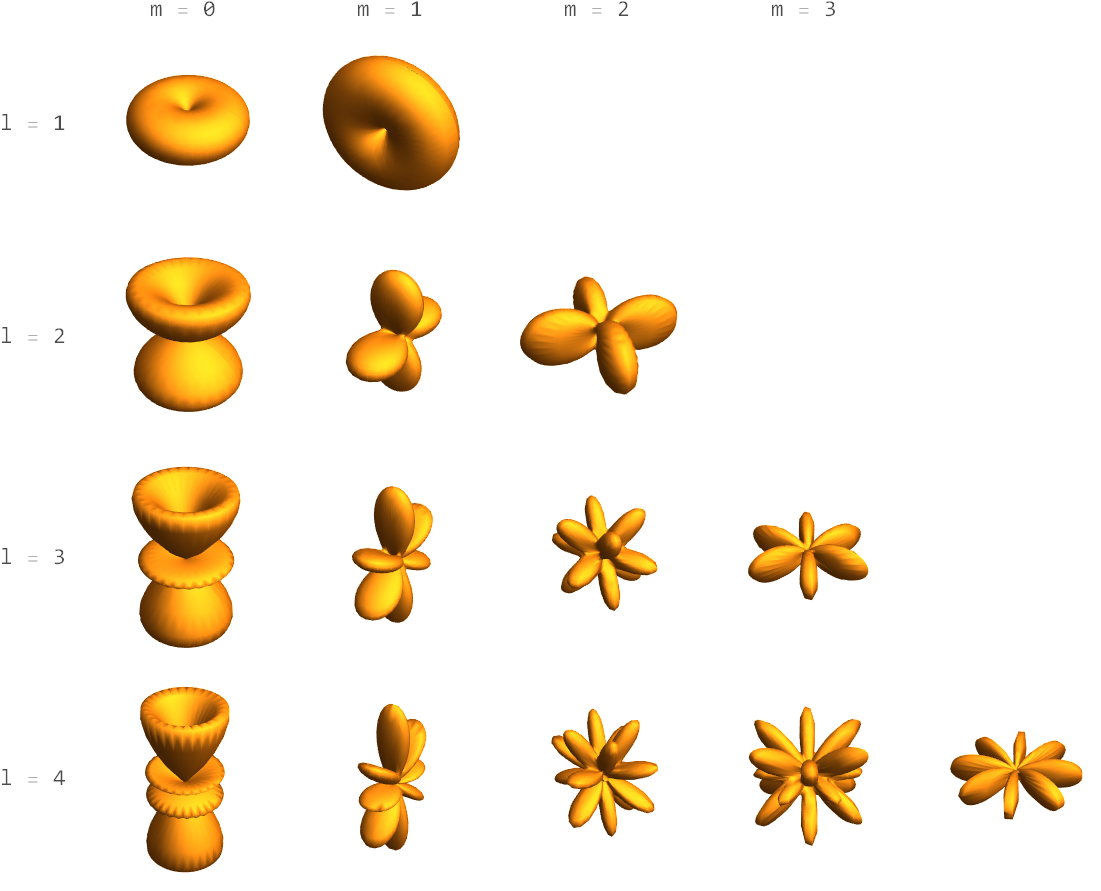
\includegraphics[width=\textwidth,height=0.6\textheight,keepaspectratio]{angle_modes_vect_ii}
            \caption[]{Векторные угловые моды для нескольких $l$ (изображена плотность энергии)}
            \label{fig:angle_modes_vect_ii}
        \end{figure}

    \end{frame}

    %
    %
    %
    %%%%%%%%%%%%%%%%%%%%%%%%%%%%%%%%%%%%%%%%%%%%%%%%%%%%%%%%%%%%%%%%%%%%%%%
    %                            FRAME                                    %
    %%%%%%%%%%%%%%%%%%%%%%%%%%%%%%%%%%%%%%%%%%%%%%%%%%%%%%%%%%%%%%%%%%%%%%%
    %
    %
    %

    \begin{frame}\frametitle{Векторные радиальные моды~--- получение}

        Уравнение \autoref{eq:wave_equation} при подстановке в него \autoref{eq:angle_modes_vect} преобразуется к виду
        %
        \begin{equation*}
            - \qty(-2 + l + l^2 - \lambda r^2) f(r) +
            4 r f'(r) + r^2 f''(r) = 0 .
        \end{equation*}
        %
        Его решение:
        %
        \begin{equation*}
            f(r) = \frac{S_l(\sqrt\lambda r)}{r^2} .
        \end{equation*}
        %
        Здесь $S_l$~--- функция Риккати-Бесселя первого рода.

    \end{frame}

    %
    %
    %
    %%%%%%%%%%%%%%%%%%%%%%%%%%%%%%%%%%%%%%%%%%%%%%%%%%%%%%%%%%%%%%%%%%%%%%%
    %                            FRAME                                    %
    %%%%%%%%%%%%%%%%%%%%%%%%%%%%%%%%%%%%%%%%%%%%%%%%%%%%%%%%%%%%%%%%%%%%%%%
    %
    %
    %

    \begin{frame}\frametitle{Векторные радиальные моды}

        \begin{figure}[h]
            \centering
            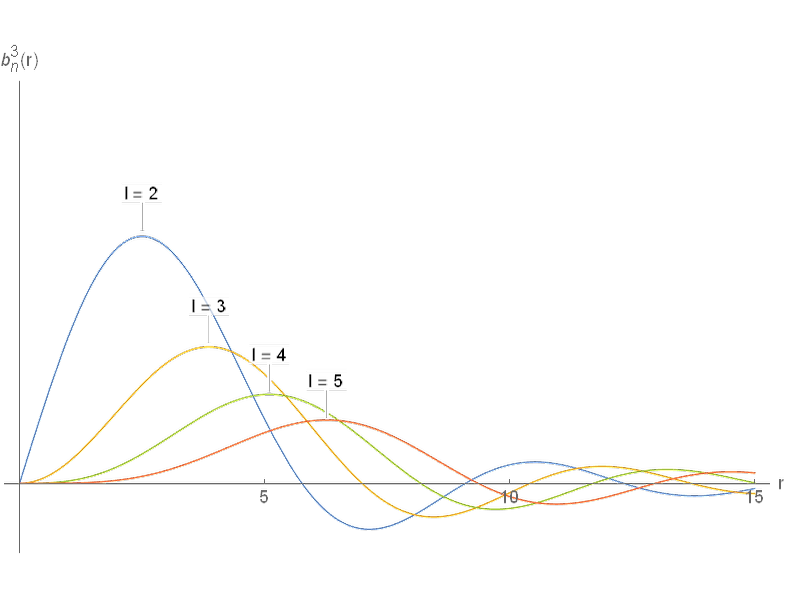
\includegraphics[width=\textwidth,height=0.6\textheight,keepaspectratio]{radial_modes_vect_ii}
            \caption[]{Векторные радиальные моды для нескольких $l$}
            \label{fig:radial_modes_vect_ii}
        \end{figure}

    \end{frame}

    %
    %
    %
    %%%%%%%%%%%%%%%%%%%%%%%%%%%%%%%%%%%%%%%%%%%%%%%%%%%%%%%%%%%%%%%%%%%%%%%
    %                            FRAME                                    %
    %%%%%%%%%%%%%%%%%%%%%%%%%%%%%%%%%%%%%%%%%%%%%%%%%%%%%%%%%%%%%%%%%%%%%%%
    %
    %
    %

    \begin{frame}\frametitle{Векторные радиальные моды~--- окончание}

        Итак, мы окончательно получили базовую моду $\vb{E}_{TE}$:
        %
        \begin{equation*}
            \vb{E}_{TE} = \begin{pmatrix}
                0 \\ 0 \\ \flatfrac{S_l(\sqrt\lambda r)}{r^2} \csc(\theta) P^1_l(\cos\theta)
            \end{pmatrix} .
        \end{equation*}
        %
        Применением ротора к ней получим $\vb{E}_{TH}$:
        %
        \begin{equation*}
            \vb{E}_{TH} = \begin{pmatrix}
                \flatfrac{l(l+1) S_l(\sqrt\lambda r)}{r^2} P_l(\cos\theta) \\
                \flatfrac{S_l'(\sqrt\lambda r)}{r^2} P_l^1(\cos\theta) \\
                0
            \end{pmatrix} .
        \end{equation*}

    \end{frame}

    %
    %
    %
    %%%%%%%%%%%%%%%%%%%%%%%%%%%%%%%%%%%%%%%%%%%%%%%%%%%%%%%%%%%%%%%%%%%%%%%
    %                            FRAME                                    %
    %%%%%%%%%%%%%%%%%%%%%%%%%%%%%%%%%%%%%%%%%%%%%%%%%%%%%%%%%%%%%%%%%%%%%%%
    %
    %
    %

    \begin{frame}\frametitle{Учет граничных условий}

        \begin{itemize}
            \item Граничные условия~--- исчезновение тангенциальной компоненты поля.

            \item Отсюда $S_l(\sqrt\lambda r_\text{шара}) = 0$ для $TE$-поляризации и $S_l'(\sqrt\lambda r_\text{шара}) = 0$ для $TH$-поляризации.

            \item $\sqrt\lambda = \flatfrac{\omega}{v}$, значит из граничных условий получим спектр собственных частот резонатора $\omega^{lp}_n$ ($p$~--- тип поляризации, $TH$ или $TE$).

            \item $\omega^{lp}_n$-й собственной частоте соответствует $2l + 1$ мод (одна базовая с $m = 0$ и $2l$ производных с $m = \pm 1, \pm 2, \dots, \pm l$).
        \end{itemize}

    \end{frame}

    %
    %
    %
    %%%%%%%%%%%%%%%%%%%%%%%%%%%%%%%%%%%%%%%%%%%%%%%%%%%%%%%%%%%%%%%%%%%%%%%
    %                            SECTION                                  %
    %%%%%%%%%%%%%%%%%%%%%%%%%%%%%%%%%%%%%%%%%%%%%%%%%%%%%%%%%%%%%%%%%%%%%%%
    %
    %
    %

    \section[СПЭ]{Построение кривой спектральной плотности энергии}

    %
    %
    %
    %%%%%%%%%%%%%%%%%%%%%%%%%%%%%%%%%%%%%%%%%%%%%%%%%%%%%%%%%%%%%%%%%%%%%%%
    %                            FRAME                                    %
    %%%%%%%%%%%%%%%%%%%%%%%%%%%%%%%%%%%%%%%%%%%%%%%%%%%%%%%%%%%%%%%%%%%%%%%
    %
    %
    %

    \begin{frame}\frametitle{Спектральная плотность энергии}

        \begin{itemize}
            \item По определению спектральной плотности энергии
            %
            \begin{equation}\label{eq:psd}
                u(\omega) \dd{\omega} = \hbar\omega\ n(\hbar\omega) \dd{N(\omega)} ,
            \end{equation}

            \item Можно показать \cite{sivuhin_opt}, что для электромагнитного поля
            %
            \begin{equation}\label{eq:dN_of_eps_cont}
                \dd{N(\omega)} = \frac{\omega^2 \dd{\omega}}{\pi^2 v^3} .
            \end{equation}

            \item Распределение Бозе-Эйнштейна:
            %
            \begin{equation}\label{eq:n_of_eps}
                n(\varepsilon) = \frac{1}{\exp(\flatfrac{\varepsilon}{kT}) - 1} .
            \end{equation}

            \item Формула Планка:
            %
            \begin{equation}
                u(\omega) = \frac{
                        \flatfrac{\omega^2 \hbar\omega}{\pi^2 v^3}
                }{\exp(\flatfrac{\hbar\omega}{kT}) - 1} .
            \end{equation}

        \end{itemize}

    \end{frame}

    %
    %
    %
    %%%%%%%%%%%%%%%%%%%%%%%%%%%%%%%%%%%%%%%%%%%%%%%%%%%%%%%%%%%%%%%%%%%%%%%
    %                            FRAME                                    %
    %%%%%%%%%%%%%%%%%%%%%%%%%%%%%%%%%%%%%%%%%%%%%%%%%%%%%%%%%%%%%%%%%%%%%%%
    %
    %
    %

    \begin{frame}\frametitle{Подсчет мод}

        \begin{itemize}
            \item В нашем случае $N(\omega^{lp}_n) = 2l + 1$.

            \item $\dv*{N(\omega)}{\omega} \approx \flatfrac{\Delta N}{\Delta \omega}$, где $\Delta N$~--- количество мод на единицу объема в спектральном интервале $\qty(\omega - \Delta\omega/2, \omega + \Delta\omega/2)$.
            %
            \begin{equation*}
                V_\text{шара} \Delta N(\omega) = \sum\limits_{
                    \qty|\omega - \omega_n| < \Delta\omega/2
                } N(\omega_n)
            \end{equation*}

        \end{itemize}

    \end{frame}

    %
    %
    %
    %%%%%%%%%%%%%%%%%%%%%%%%%%%%%%%%%%%%%%%%%%%%%%%%%%%%%%%%%%%%%%%%%%%%%%%
    %                            FRAME                                    %
    %%%%%%%%%%%%%%%%%%%%%%%%%%%%%%%%%%%%%%%%%%%%%%%%%%%%%%%%%%%%%%%%%%%%%%%
    %
    %
    %

    \begin{frame}

        \begin{figure}[h]
            \centering
            %
            \subfloat[][]{%
                \label{fig:n_full}%
                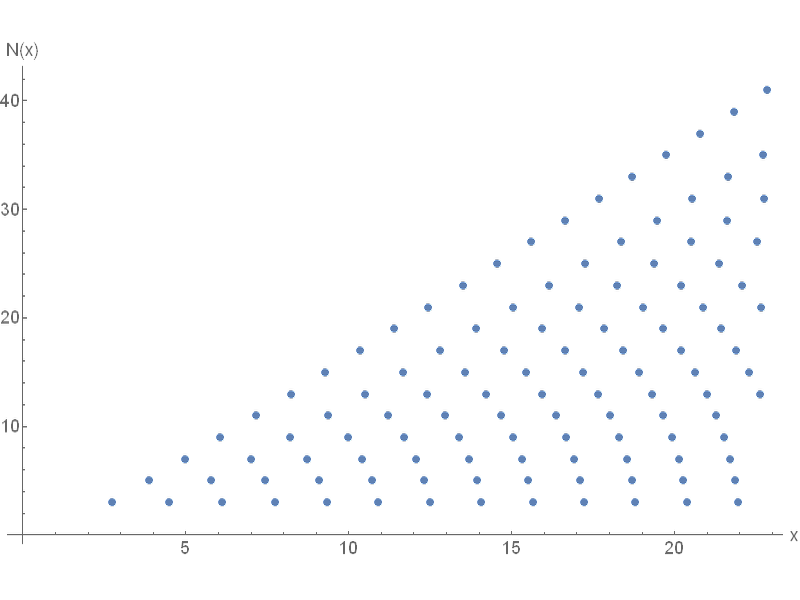
\includegraphics[width=0.45\textwidth]{n_full}}%
            \hspace{8pt}%
            %
            \subfloat[][]{%
                \label{fig:dndx_mag}%
                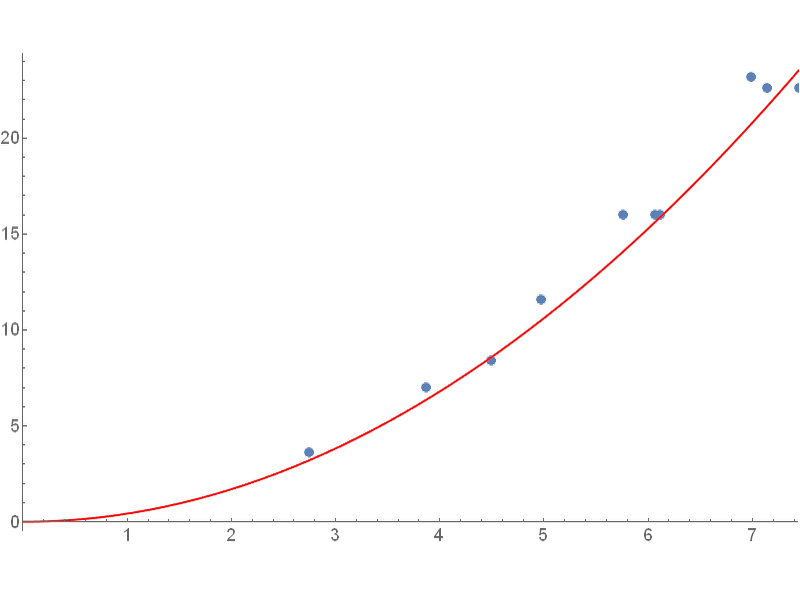
\includegraphics[width=0.45\textwidth]{dndx_mag}}%
            \hspace{8pt}%
            %
            \caption[]{$N(x_n)$ и $\flatfrac{\Delta N}{\Delta x}$ вблизи нуля, $x = \flatfrac{\omega}{v} r_\text{шара}$}
        \end{figure}

    \end{frame}

    %
    %
    %
    %%%%%%%%%%%%%%%%%%%%%%%%%%%%%%%%%%%%%%%%%%%%%%%%%%%%%%%%%%%%%%%%%%%%%%%
    %                            FRAME                                    %
    %%%%%%%%%%%%%%%%%%%%%%%%%%%%%%%%%%%%%%%%%%%%%%%%%%%%%%%%%%%%%%%%%%%%%%%
    %
    %
    %

    \begin{frame}

        \begin{figure}[h]
            \centering
            %
            \subfloat[][]{%
                \label{fig:dndx}%
                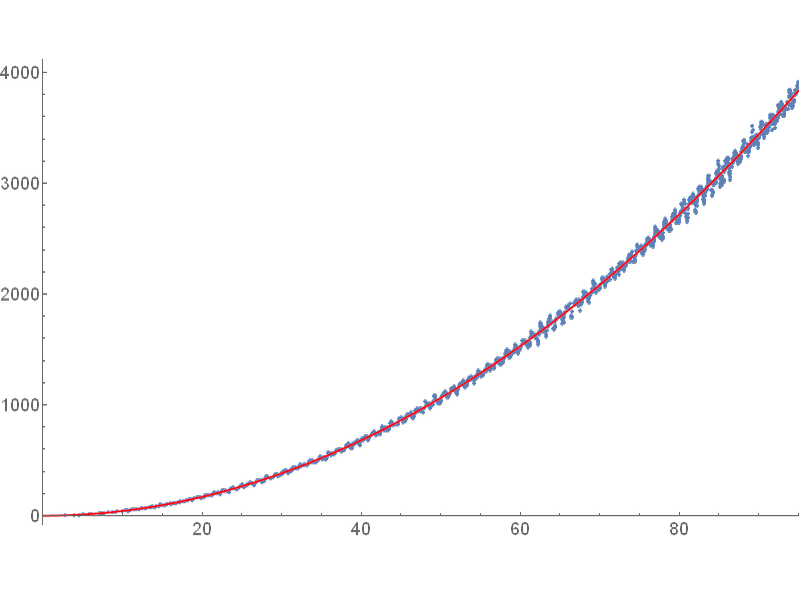
\includegraphics[width=0.45\textwidth]{dndx}}%
            \hspace{8pt}%
            %
            \subfloat[][]{%
                \label{fig:plank}%
                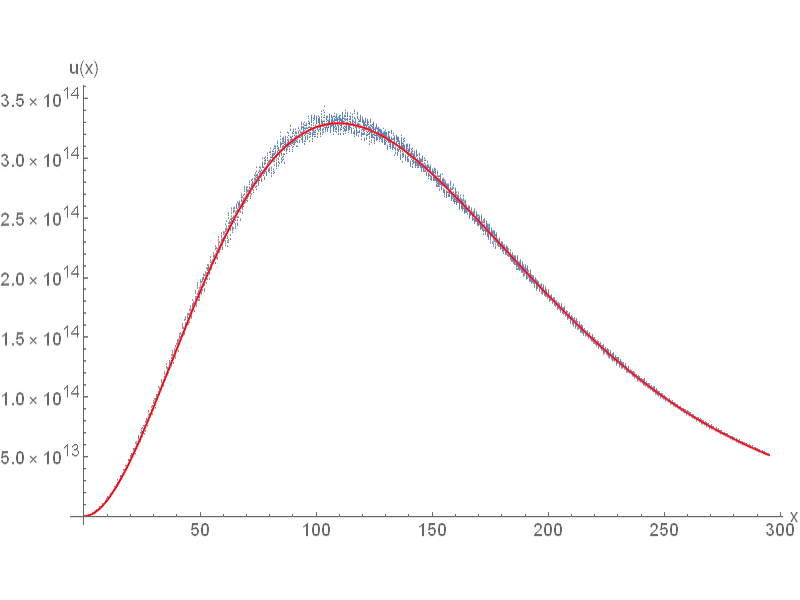
\includegraphics[width=0.45\textwidth]{plank}}%
            \hspace{8pt}%
            %
            \caption[]{$\flatfrac{\Delta N}{\Delta x}$ и $u(x)$ в б\'{о}льшем интервале частот, $x = \flatfrac{\omega}{v} r_\text{шара}$}
        \end{figure}

    \end{frame}

    %
    %
    %
    %%%%%%%%%%%%%%%%%%%%%%%%%%%%%%%%%%%%%%%%%%%%%%%%%%%%%%%%%%%%%%%%%%%%%%%
    %                            SECTION                                  %
    %%%%%%%%%%%%%%%%%%%%%%%%%%%%%%%%%%%%%%%%%%%%%%%%%%%%%%%%%%%%%%%%%%%%%%%
    %
    %
    %

    \section{Заключение}

    %
    %
    %
    %%%%%%%%%%%%%%%%%%%%%%%%%%%%%%%%%%%%%%%%%%%%%%%%%%%%%%%%%%%%%%%%%%%%%%%
    %                            FRAME                                    %
    %%%%%%%%%%%%%%%%%%%%%%%%%%%%%%%%%%%%%%%%%%%%%%%%%%%%%%%%%%%%%%%%%%%%%%%
    %
    %
    %

    \begin{frame}\frametitle{Заключение}

        \begin{itemize}
            \item В работе продемонстрировано применение методики Ли-генерации мод скалярного и векторного полей в трехмерном евклидовом пространстве.

            \item Математические выкладки проделаны для риманова пространства общего вида.

            \item Получен вид скалярных и векторных сферических мод.

            \item Построена кривая спектральной плотности запасенной в резонаторе энергии.
        \end{itemize}

        Все поставленные цели были достигнуты.

    \end{frame}

    %
    %
    %
    %%%%%%%%%%%%%%%%%%%%%%%%%%%%%%%%%%%%%%%%%%%%%%%%%%%%%%%%%%%%%%%%%%%%%%%
    %                        BIBLIOGRAPHY                                 %
    %%%%%%%%%%%%%%%%%%%%%%%%%%%%%%%%%%%%%%%%%%%%%%%%%%%%%%%%%%%%%%%%%%%%%%%
    %
    %
    %

    \begin{frame}\frametitle{Литература}
        \bibliographystyle{../../../lib/doc/bib/utf8gost705s}
        \bibliography{%
            ../../../lib/doc/bib/resonators,%
            ../../../lib/doc/bib/physics,%
            ../../../lib/doc/bib/math%
        }
    \end{frame}

\end{document}
